\section{最佳N项逼近}
\label{sec:fapprox-best-n-term}

固定子空间对所有目标一视同仁：截断Fourier级数总是保留低频，固定网格总是在同样的位置细分。目标的重要信息若集中在少数几个预先没有选中的方向上，固定选法就会浪费预算。本节仍固定一组完备标准正交基，但允许根据目标挑选保留哪些基向量，只限制挑选的个数。

先用一个向量看这件事。在$\mathbb R^5$中取
\[
 v=(0.1,\ 3,\ -0.2,\ 2,\ 0.4).
\]
若只能留两个坐标，总是留前两个的话，被舍弃的是$-0.2,2,0.4$，平方误差是$0.04+4+0.16=4.2$。若留绝对值最大的两个，即$3$和$2$，被舍弃的是$0.1,-0.2,0.4$，平方误差只有$0.21$。同样的预算，差了二十倍。

设$H$是可分Hilbert空间，$(e_n)_{n\geq1}$是一组标准正交基，$f$的系数为$c_n=\langle e_n,f\rangle$。对预算$N$，令
\[
 \Sigma_N=\Bigl\{\sum_{n\in\Lambda}a_ne_n:\ \Lambda\subseteq\mathbb N,\ \lvert\Lambda\rvert\leq N,\ a_n\in\mathbb K\Bigr\}.
\]

\begin{definition}[最佳N项逼近]
\label{def:fapprox-best-n-term}
称
\begin{equation}
 \sigma_N(f)_2=E(f,\Sigma_N)_H=\inf_{g\in\Sigma_N}\lVert f-g\rVert
 \label{eq:fapprox-best-n-term}
\end{equation}
为$f$关于基$(e_n)$的最佳$N$项误差；达到这个下确界的元素称为$f$的\term{最佳N项逼近}（best N-term approximation）。
\end{definition}

$\Sigma_N$是第~\ref{sec:fapprox-budget}节所说的非线性候选集合。它是所有至多$N$维坐标子空间的并，两个元素之和可能用到$2N$个基向量；图~\ref{fig:fapprox-nearest-point}(c)画的正是$\mathbb R^2$中的$\Sigma_1$。非线性只来自支撑集合$\Lambda$依赖于目标，一旦$\Lambda$选定，近似就是在线性子空间$\operatorname{span}\{e_n:n\in\Lambda\}$中作正交投影。

\subsection{固定截断与自适应选择}
\label{sec:fapprox-fixed-vs-adaptive}

在同一组基和同一个项数下比较两种做法。固定截断预先规定下标集合$\Lambda_N=\{1,\ldots,N\}$，对所有目标都保留前$N$项，误差为
\[
 \Bigl(\sum_{n>N}\lvert c_n\rvert^2\Bigr)^{1/2},
\]
这是第~\ref{sec:fapprox-fixed-space}节在$V_N=\operatorname{span}\{e_1,\ldots,e_N\}$中的最佳逼近。自适应选择则对每个目标分别挑选$\Lambda$。由定义，$\sigma_N(f)_2$不超过固定截断的误差，差距取决于大系数是否恰好排在前面。

极端情形下差距可以达到最大。取$f=e_{N+1}$，固定截断的误差为$\lVert f\rVert=1$，而一项就能精确表示它，$\sigma_1(f)_2=0$。不那么极端的情形同样常见：一个大部分区域光滑、只在某处有跳跃的函数，在小波基中的大系数集中在跳跃附近的细尺度上，按“先粗后细、从左到右”的固定次序要保留许多无用的系数才能轮到它们。

自适应选择的代价是需要知道系数的大小。要挑出重要的系数，通常得先计算或估计足够多的系数，再按大小筛选；被挑出的下标集合也要存储，它本身就是表示的一部分。所以最佳$N$项误差衡量的是“已知全部系数时用$N$项能做到多好”，它与在有限计算下找到这些项的问题是两回事。

\subsection{最大系数选择}
\label{sec:fapprox-largest-coefficients}

在正交基和$L^2$型范数下，最佳$N$项逼近有简单的显式解。由$f\in H$，$\sum_n\lvert c_n\rvert^2<\infty$，所以对任意$t>0$，满足$\lvert c_n\rvert\geq t$的下标只有有限个。于是可以把系数的绝对值按非增次序排列为
\[
 c_1^*\geq c_2^*\geq\cdots
\]
相等的值任意排序，非零系数有限时在末尾补零。

\begin{theorem}[保留最大系数最优]
\label{thm:fapprox-largest-coefficients}
设$\Lambda_N^*$是$\lvert c_n\rvert$最大的$N$个下标组成的集合，$g_N=\sum_{n\in\Lambda_N^*}c_ne_n$。则$g_N$是$f$的最佳$N$项逼近，并且
\begin{equation}
 \sigma_N(f)_2^2=\sum_{n>N}(c_n^*)^2 .
 \label{eq:fapprox-largest-coefficients}
\end{equation}
\end{theorem}

\begin{proof}
任取$\lvert\Lambda\rvert\leq N$与系数$a_n$，令$g=\sum_{n\in\Lambda}a_ne_n$。由Parseval等式，$f-g$的平方范数按坐标拆开：
\[
 \lVert f-g\rVert^2=\sum_{n\in\Lambda}\lvert c_n-a_n\rvert^2+\sum_{n\notin\Lambda}\lvert c_n\rvert^2 .
\]
第一项非负，在$a_n=c_n$时为零。所以对固定的$\Lambda$，最好的系数就是原系数，于是
\[
 \lVert f-g\rVert^2\geq\sum_{n\notin\Lambda}\lvert c_n\rvert^2=\lVert f\rVert^2-\sum_{n\in\Lambda}\lvert c_n\rvert^2 .
\]

$\Lambda$至多含$N$个下标，$\sum_{n\in\Lambda}\lvert c_n\rvert^2$不超过最大的$N$个平方之和，等号在$\Lambda=\Lambda_N^*$时取到。所以
\[
 \lVert f-g\rVert^2\geq\lVert f\rVert^2-\sum_{n\leq N}(c_n^*)^2=\sum_{n>N}(c_n^*)^2 ,
\]
而$g_N$达到这个下界。
\end{proof}

证明依赖两件事。第一，误差平方能拆成各方向上的平方和，这来自基的正交性和Parseval等式。第二，这种拆分让“选哪些方向”与“选什么系数”分开处理。若基不正交，或使用冗余的字典，同一个函数有多种展开，系数本身不唯一，误差也不再是舍弃系数的平方和。

换一把尺子同样会出问题。用下面的Haar基，取$f=1.2\varphi+\psi_{2,0}$，一致范数下比较保留哪一项。$\psi_{2,0}$在$[0,\frac18)$上取$2$、在$[\frac18,\frac14)$上取$-2$，其余为零。按最大系数规则保留系数$1.2$的$\varphi$，则对任何$a$，$f-a\varphi$在这两段上相差$4$，所以
\[
 \lVert f-a\varphi\rVert_\infty\geq2 .
\]
改为保留系数较小的$\psi_{2,0}$，误差只有$\lVert1.2\varphi\rVert_\infty=1.2$。原因是细尺度的基函数高而窄，系数小但一致范数大。

\paragraph{Haar展开中的选择}
用第~\ref{chap:wavelet-transform}章的Haar基复算这一选择。在$L^2(0,1)$上，记
\[
 \varphi=\mathbf 1_{[0,1)},\qquad \psi=\mathbf 1_{[0,1/2)}-\mathbf 1_{[1/2,1)},\qquad \psi_{j,k}(x)=2^{j/2}\psi(2^jx-k),
\]
其中$j\geq0$，$0\leq k<2^j$；$\varphi$与全体$\psi_{j,k}$组成标准正交基。取在$3/4$处向下跳跃的阶梯函数
\[
 f=3\cdot\mathbf 1_{[0,3/4)}-\mathbf 1_{[3/4,1)} .
\]

逐个计算内积。$\varphi$的系数就是平均值：
\[
 \langle\varphi,f\rangle=\frac{3\cdot3-1}4=2 .
\]
$\psi_{0,0}$的系数是左半积分减右半积分：
\[
 \langle\psi_{0,0},f\rangle=\int_0^{1/2}f-\int_{1/2}^1f=\frac32-\frac12=1 .
\]
下一层的两个系数分别是
\[
 \langle\psi_{1,0},f\rangle=0,\qquad
 \langle\psi_{1,1},f\rangle=\sqrt2\Bigl(\int_{1/2}^{3/4}f-\int_{3/4}^1f\Bigr)=\sqrt2 .
\]
$j\geq2$时，$\psi_{j,k}$支撑在某个长为$1/4$的二进区间内且积分为零，$f$在这样的区间上是常数，内积为零。

于是$f$只有三个非零坐标：
\[
 f=2\varphi+\psi_{0,0}+\sqrt2\,\psi_{1,1}.
\]
用Parseval等式检验：$\lVert f\rVert^2=(9\cdot3+1)/4=7$，而$2^2+1^2+(\sqrt2)^2=7$。

按“先粗后细、同层从左到右”的固定次序$\varphi,\psi_{0,0},\psi_{1,0},\psi_{1,1},\ldots$截断，保留两项得$2\varphi+\psi_{0,0}$，误差平方为$2$；保留三项仍缺$\psi_{1,1}$，误差平方仍为$2$。系数绝对值的非增排列是$2,\sqrt2,1,0,\ldots$，由定理~\ref{thm:fapprox-largest-coefficients}，最佳两项逼近为$2\varphi+\sqrt2\,\psi_{1,1}$，误差平方为
\[
 \sigma_2(f)_2^2=1 .
\]
最佳三项逼近就是$f$本身，$\sigma_3(f)_2=0$。

图~\ref{fig:fapprox-best-n-term}对照了两种选择。固定次序的近似在跳跃所在的右半区间上偏差最大；最佳两项逼近把预算用到了$\psi_{1,1}$，正好捕捉到跳跃，代价是在左半区间留下幅度为$1$的偏差。跳跃位于右半区间的细尺度上，固定次序先用掉了左半区间那个为零的系数，自适应选择直接找到了它。

\begin{BookInlineFigure}
  \centering
  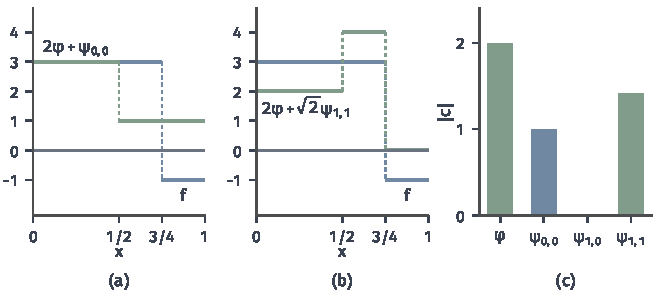
\includegraphics[width=112mm]{figures/04-spaces-measures-and-geometry/03-function-spaces/matplotlib/fapprox-best-n-term/figure.pdf}
  \caption{同一预算下的两种选择。目标$f$（蓝）在$3/4$处跳跃，均保留两项（绿）。(a)固定次序保留$\varphi,\psi_{0,0}$，误差平方为$2$。(b)保留系数最大的$\varphi,\psi_{1,1}$，误差平方为$1$。(c)前四个Haar系数的绝对值，绿色为最佳两项选中的系数；固定次序选的是前两根柱子。}
  \label{fig:fapprox-best-n-term}
\end{BookInlineFigure}
